% Apéndice Laminado y trenes de laminación

\chapter{Laminado y trenes de laminación.} % Main appendix title

\label{AppendixLaminacionYTrenes} % For referencing this appendix elsewhere, use \ref{AppendixA}


%\section{Laminado y trenes de laminación.}

El laminado, conocido como \textit{rolling} en inglés es un proceso metalurgico que consiste en conformar un material haciendo que una o dos de sus dimensiones sean mucho mayores que las restantes. En forma industrial esto se consigue haciendo pasar al material a través de  rodillos separados entre sí una distancia menor que el espesor inicial del material sometiéndolo simultáneamente a compresión y estiramiento. 


\section{Jaulas de laminación.}

Las máquinas de laminar cuando son de una sola etapa se conocen como \emph{laminadoras} y cuando tiene varias etapas se conocen como \emph{trenes de laminacion} o \textit{rolling mills} en inglés. El elemento básico para laminar se conoce con el nombre de \emph{jaula}  o \emph{caja} y se compone de los cilindros y de una estructura que sirve de soporte llamada castillete. El tren de laminación comprende al conjunto de jaulas y todos los demás elementos auxiliares que permiten su gobierno y regulación tales como los motores de accionamiento de los cilindros las mesas de rodillos para la entrada y salida del material, las cizallas, etcétera.



La jaula podrá estar constituida por dos o más cilindros horizontales, un bastidor que soporta los asientos de los cilindros y un sistema de ajuste formado por espárragos roscados. Las jaulas serán reversibles si los cilindros pueden girar en ambos sentidos haciendo pasar el material alternativamente de ida y vuelta. Las jaulas trío no reversibles disponen de tres cilindros en un mismo plano la laminación ocurre alternativamente un sentido con los cilindros medio e inferior y en el contrario en los cilindros medio y superior.

Cuando se pretenden grandes reducciones es preciso ejercer fuertes presiones. Para ello se utilizan las jaulas cuarto que disponen de dos juegos de cilindros: el primero (los cilindros de trabajo) de pequeño diámetro, entre los que pasa el material que se quiere laminar; sobre éstos se apoya el segundo juego (los cilindros de apoyo) de mayor diámetro, que transmiten el esfuerzo a los de trabajo. Una jaula cuarto puede ser reversible. Actualmente la tecnología a llevado el número de cilindros por jaula en diversas configuraciones hasta veinte.

Si se desea obtener un producto de muy pequeño espesor la longitud final es tal que no es posible emplear un tren reversible de una sola caja por la gran longitud del producto acabado (las velocidades pueden llegar  a los 50 m/s) y porque el material se enfría en las largas pasadas sucesivas. El problema se resuelve haciendo pasar el material por varias cajas en cascada que se llama \emph{tren continuo}, donde el producto es laminado sucesivamente en varias jaulas, consecutivas.

La superficie de los rodillos se llama tabla y puede ser lisa o acanalada según:

\begin{itemize}
	\item Planos. Rodillos planos paralelos de gran sección usados para hacer láminas planas (chapas) de distintos espesores como producto final.
	\item Conformados. Rodillos planos de sección pequeña dispuestos en formas alabeadas usados para crear perfiles de pequeño espesor plegando láminas planas.
	\item Perfilados. Rodillos con laterales perfilados por lo general complementarios usados para crear figuras de gran espesor conformando barras rectangulares. Esto también es conocido como \emph{laminado de forma}.
\end{itemize}

En todos los casos se modifica la sección transversal del material a base de reducir su espesor.



\section{Trenes de laminación en caliente.}

El laminado en caliente es un proceso de trabajo del metal que ocurre por encima de la temperatura de recristalización del material. Después de que los granos se deforman durante el procesamiento, se recristalizan, lo que mantiene una microestructura equitaxial y evita que el metal se endurezca. El material de partida suele ser grandes piezas de fundición semiacabadas conocidas como losas y palanquillas. Si las piezas provienen de una operación de colada continua éstas se alimentan directamente a los laminadores a la temperatura adecuada. En operaciones pequeñas, el material comienza a temperatura ambiente y debe calentarse previamente; si las piezas son de grandes dimensiones se hace en hornos a gas o petróleo. Si las piezas a trabajar son pequeñas se utiliza calentamiento por inducción. A medida que se trabaja el material, se debe controlar la temperatura para asegurarse de que permanece por encima de la temperatura de recristalización. Para mantener un factor de seguridad se define una temperatura de acabado de 50 a 100 \textdegree C por encima de la temperatura de recristalización. Si la temperatura desciende por debajo de esta temperatura el material debe ser calentado nuevamente antes de la laminación.

Los metales laminados en caliente generalmente no tienen gran direccionalidad en sus propiedades mecánicas ni grandes tensiones residuales inducidas por deformación. Sin embargo en ciertos casos las inclusiones no metálicas imparten algo de direccionalidad y las piezas trabajadas en caliente de menos de 20 mm de espesor suelen tener algunas propiedades direccionales.
El gran problema suele provenir del enfriamiento no uniforme que produce tensiones residuales importantes, particularmente en perfiles que tienen una sección transversal no uniforme como las vigas en I. Los productos directamente salidos del tren son de buena calidad pero la superficie está cubierta por óxidos negros que se forman a altas temperaturas. Éstos se suelen eliminar mediante un decapado químico o procesos de remoción mecánica. Las tolerancias dimensionales son del 2 al 5\% de las dimensiones totales.

El laminado en caliente se utiliza principalmente para producir rollos y láminas de metal usadas como insumos de otras industrias, también planchas para construcciones navales y secciones transversales simples, como vigas de construcción, vías ferroviarias, guardarraíles, etcétera. En la figura \ref{fig:hot-steel-rolling-mill} podemos ver detalles de un tren de laminación de siete jaulas y varios juegos de rodillos

\begin{figure}[h]
	\centering
	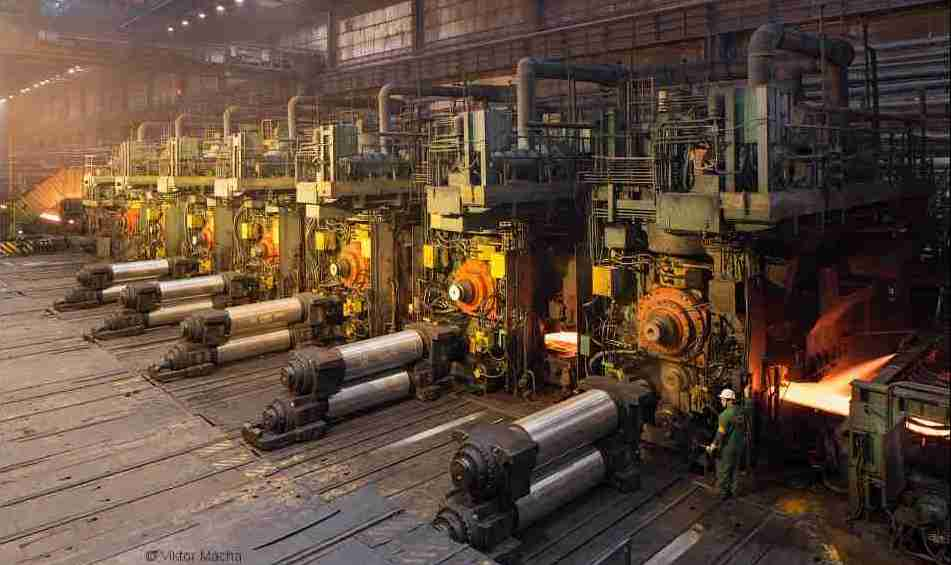
\includegraphics[width=0.90\textwidth]{./Figures/nlmk-lipetsk-dokoncovaci-stojany-na-valcovne-pasu-1793-r2.jpg}
	\caption{tren de laminación en caliente con detalle de los rodillos\protect\footnotemark.}
	\label{fig:hot-steel-rolling-mill}
\end{figure}.
\footnotetext{\url{https://www.viktormacha.com/klicova-slova/nlmk-lipetsk-finishing-stand-at-the-hot-1793.html}}

Los laminadores se dividen en jaulas de desbaste, intermedias y de acabado. Durante el laminado de forma, una palanquilla inicial (redonda o cuadrada) con un borde de diámetro que generalmente varía entre 100 y 140 mm se deforma continuamente para producir cada producto terminando con dimensiones y geometría de sección transversal más pequeñas. Se pueden adoptar diferentes secuencias para producir un determinado producto final a partir de un tocho dado. Sin embargo, dado que cada jaula del laminador es sumamente costosa (del orden de los millones de dólares) un requisito típico es limitar en todo lo posible el número de pases de laminación al que debe someterse la pieza.


\begin{figure}[h]
	\centering
	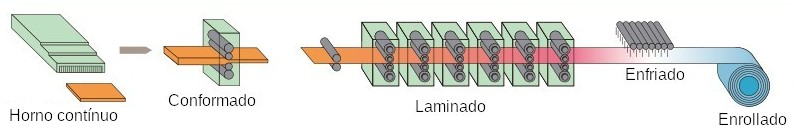
\includegraphics[width=0.99\textwidth]{./Figures/EsquemaLaminadoCalienteFinal.jpg}
	\caption{Esquema de tren de laminación en caliente.}
	\label{fig:EsquemaLaminadoCaliente}
\end{figure}


\section{Trenes de laminación en frío.}\label{cap:MetBas}
La laminación en frío ocurre con el metal por debajo de su temperatura de recristalización (generalmente a temperatura ambiente), lo que aumenta la resistencia mediante endurecimiento por deformación hasta un 20\%, también mejora el acabado de la superficie y mantiene tolerancias más estrictas. Los productos comúnmente laminados en frío incluyen láminas, tiras, barras y varillas, pero más pequeños que los mismos productos que laminados en caliente. En cada pasada de laminación no se puede reducir el espesor tanto como la laminación en caliente y las altas presiones y esfuerzos longitudinales hacen que las jaulas y los rodillos deban tener configuraciones especiales.

En la figura \ref{fig:tren_frio_01} podemos ver el detalle de las estaciones por las que pasa el acero en un tren de laminación en frío. En lo que a nuestro proyecto interesa, en la estación \textbf{B} se encuentra el dispositivo que alinea los cantos de la cola del rollo de chapa que se termina con el canto del comienzo del nuevo rollo a través de dos prensas hidráulicas que los manipulan hasta dejarlos paralelos, luego se sueldan y se examinan. Ésto debe hacerse mientras dura el acero que se encuentra en el \textit{Buffer} de entrada \textbf{C}.

\begin{figure}[h]
	\centering
	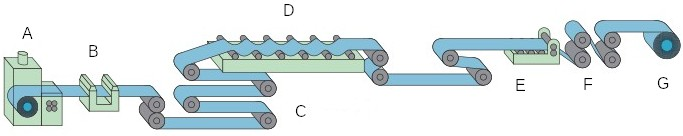
\includegraphics[width=0.99\textwidth]{./Figures/tren_frio_01.jpg}
	\caption{Esquemático tren de laminación en frío.}
	\label{fig:tren_frio_01}
\end{figure}


\begin{itemize}
	\item \textbf{A} - Desenrrolladora y cizalladora
	\item \textbf{B} - Empalmadora y soldadora
	\item \textbf{C} - \textit{Buffer} para dar tiempo a empalmar nuevos rollos
	\item \textbf{D} - \textit{pickling line} de tratamiento superficial - decapado
	\item \textbf{E} - Limitadora y alisadora
	\item \textbf{F} - Jaulas de laminado en frío
	\item \textbf{G} - Enrrolladora
\end{itemize}

El material laminado en frío viene en varias categorias: duro, semiduro, un cuarto de dureza y laminado superficial o \textit{skin rolled}. El material duro ha experimentado una reducción de espesor del 50\%, mientras que los demás lo hacen en una proporción menor. Si se desea aumentar la ductilidad se continúa con un proceso de recocido. El laminado superficial o \textit{skin rolled} es el de menor reducción: 0.5–1\% y se aplica si se desea producir una superficie lisa, un grosor uniforme y reducir el punto de fluencia creando en la superficie una alta densidad de dislocaciones no fijadas en la matriz de ferrita. Esto evita que se formen bandas de Lüders\footnote{\url{https://en.wikipedia.org/wiki/Lüders\_band}} en mecanizados posteriores. El material tratado por \textit{skin rolled} se usa en procesos de trabajo en frío donde se requiere una buena ductilidad.

En la figura \ref{fig:Tren_laminado_frio} podemos ver el detalle de las estaciones \textbf{D}, \textbf{E} y \textbf{F}. 

\begin{figure}[h]
	\centering
	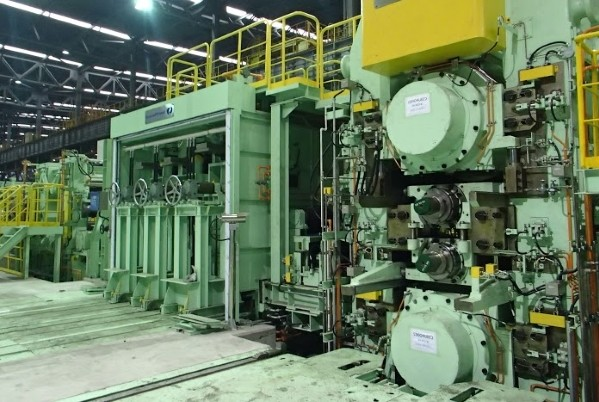
\includegraphics[width=0.90\textwidth]{./Figures/Tren_laminado_frio_SPM_s.jpg}
	\caption{Tren de laminación en frío.\protect\footnotemark.}
	\label{fig:Tren_laminado_frio}
\end{figure}
\footnotetext{\url{https://www.andritz.com/products-en/group/metals/rolling-mills/cold-rolling-mill-intermediate-rolls}}


Se pueden laminar en frío gran variedad de perfiles si la sección es uniforme y la dimensión transversal pequeña. Los perfiles laminados en frío requieren una serie de operaciones de conformado a lo largo de jaulas de: dimensionamiento, acomodado, desbaste grueso, desbaste fino, semiacabado y acabado.

En lo que hace específicamente al proceso de laminado, la principal diferencia con la laminación en caliente se encuentra en la ingeniería de las jaulas y los rodillos para evitar las deformaciones y los pandeos debido al incremento de dureza en el material. En las jaulas se disponen en serie grupos de rodillos sucesivos que reciben y distribuyen la presión ejercida sobre la chapa dirigiéndola desde ella hacia rodillos de mayor tamaño que tienen los rodamientos dimensionados para soportar los esfuerzos de compresión necesarios. Tal como lo podemos apreciar en la figura \ref{fig:cold_roll_mill_01}. 

\begin{figure}[h]
	\centering
	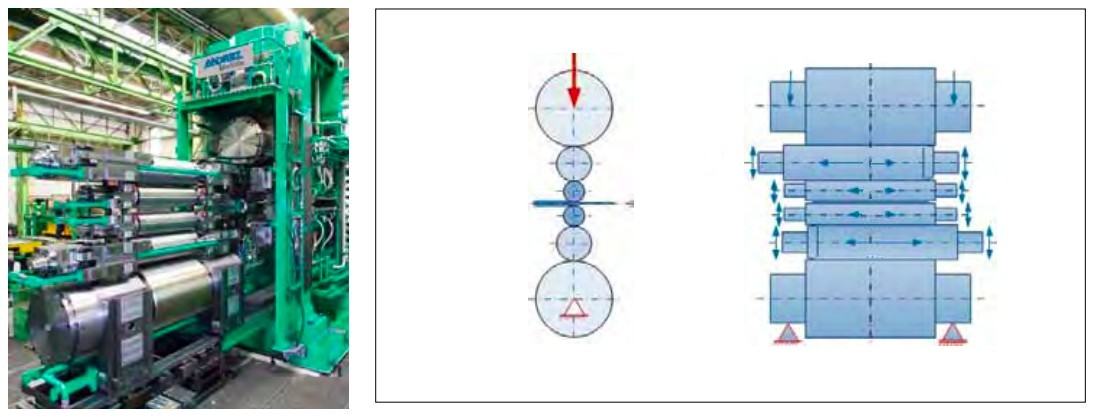
\includegraphics[width=0.99\textwidth]{./Figures/cold_roll_mill_01.jpg}
	\caption{Jaula de laminación en frío con detalle de los rodillos. El superior es el conductor y el que fija el espesor\protect\footnotemark.}
	\label{fig:cold_roll_mill_01} 
\end{figure}
\footnotetext{\url{https://www.andritz.com/resource/blob/19240/3de0e6a13dc00c213d679869d5bd9bce/me-cold-rolling-technology-carbon-en-data.pdf}}

Vemos que solo el primero de los rodillos de gran diámetro es conductor y junto con su complementario inferior transmiten los esfuerzos a la estructura de la jaula. Todos los demás rodillos son conducidos por los más externos y en sus bujes se ejercen pocos esfuerzos transversales significativos. 

Esta disposición de rodillos puede escalar verticalmente o extenderse radialmente dando lugar a complejas ingenierías de rodillos conductores y conducidos. En la figura \ref{fig:rodillosLaminadoFrio} podemos ver como la configuración de 20 rodillos se encuentra totalmente contenida radialmente y ninguno de los rodillos conducidos ejerce esfuerzos transversales.


\begin{figure}[h]
	\centering
	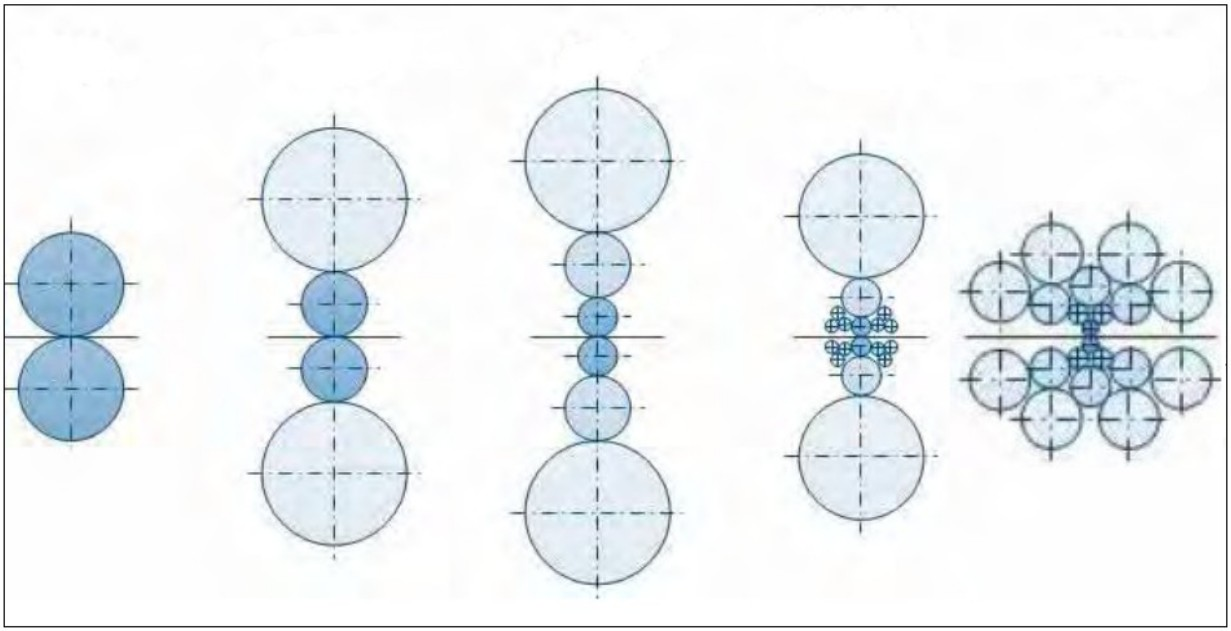
\includegraphics[width=0.75\textwidth]{./Figures/rodillos.jpg}
	\caption{Distintas configuraciones de 2, 4, 6, 6+6 y 20 rodillos\protect\footnotemark.}
	\label{fig:rodillosLaminadoFrio} 
\end{figure}
\footnotetext{\url{https://www.andritz.com/products-en/group/metals/rolling-mills/sundwig-20-high-cold-rolling-mill}}

En la figura \ref{fig:rodillosLaminadoFrio20} vemos como se implementa mecánicamente la jaula y los rodillos de la laminadora de 20 elementos. Podemos apreciar que los rodillos conducidos se encuentran libres de bujes. La jaula tiene un cierre frontal que impide  desplazamientos longitudinales de los rodillos. 

\begin{figure}[h]
	\centering
	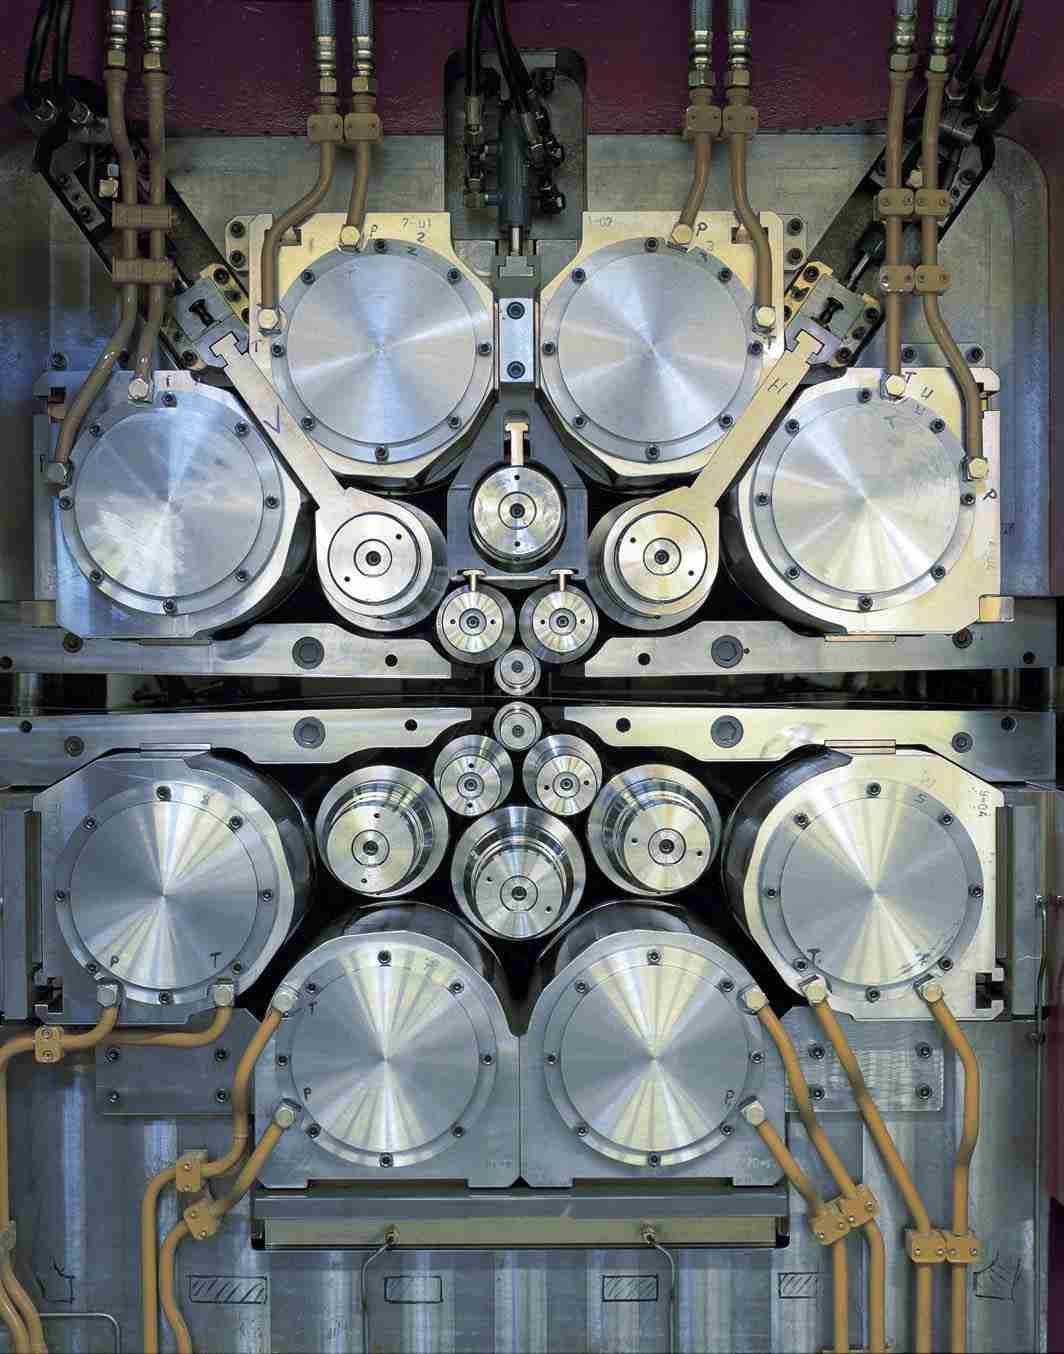
\includegraphics[width=0.75\textwidth]{./Figures/multicilindros1a.jpg}
	\caption{configuracion de 20 rodillos para laminado en frío\protect\footnotemark.}
	\label{fig:rodillosLaminadoFrio20} 
\end{figure}
\footnotetext{\url{https://www.andritz.com/products-en/group/metals/rolling-mills/sundwig-20-high-cold-rolling-mill}}

Los usos típicos del acero laminado en frío incluyen: mueblería metálica, gabinetes y hardware de computadoras, electrodomésticos y componentes, accesorios de iluminación, elementos de ferretería, bisagras, tubos, tambores de acero, cortadoras de césped, gabinetes electrónicos, calefones y termotanques, contenedores de metal, aspas de ventilador, \textit{kits} de cocina, etcétera.



\section{Soldadura en trenes de laminación.}

Mientras que el acero producido en caliente puede ser producido casi en forma contínua y ser bobinado en espesores cercanos a los 3mm en espera de darle un destino final; el acero laminado en frío se hace sobre pedido o con stock controlado, sabiéndose de antemano su destino final. Cuando se decide la producción de una tanda se hace con un destino específico y el acero original sigue el proceso explicado en \fullref{cap:MetBas} alimentándose con rollos de acero laminado en caliente. 

\subsection{Proceso de soldado.}


En las estaciones \textbf{A} y \textbf{B} el acero que ingresa al tren de laminación debe ser desenrrollado, cizallado, posicionado, empalmado y soldado. Podemos ver el posicionador enfrentando dos cantos de acero en la figura \ref{fig:posicionador}. 

\begin{figure}[h]
	\centering
	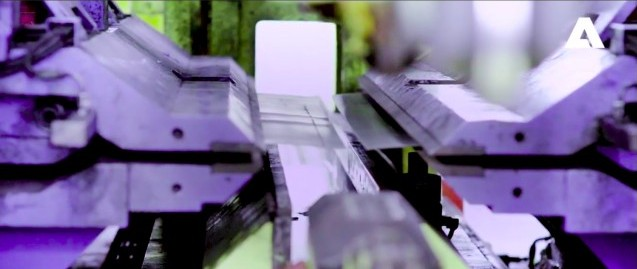
\includegraphics[width=0.90\textwidth]{./Figures/posicionador01.jpg}
	\caption{Posicionador para empalme y soldadura\protect\footnotemark.}
	\label{fig:posicionador} 
\end{figure}
\footnotetext{\url{https://youtu.be/u6hIaRdXleE?list=PLDD7zo2J8P3fcZPL6RioW2hyscS1Okfh2&t=78}}


\textbf{El proceso completo de soldado consta de las siguientes etapas:}

%Los ítemes se los puede cambiar ejecutando uno de los siguientes comandos
%\renewcommand{\labelenumi}{\arabic{enumi}.} (1., 2., 3.,…)
%\renewcommand{\labelenumi}{\roman{enumi}.} (i., ii., iii.,…)
%\renewcommand{\labelenumi}{\Roman{enumi}.} (I., II., III.,…)
%\renewcommand{\labelenumi}{\alph{enumi}.} (a., b., c.,…)
%\renewcommand{\labelenumi}{(\alph{enumi}).} [(a), (b), (c),…]
%\renewcommand{\labelenumi}{\Alph{enumi}.} (A., B., C.,…)
\begin{enumerate}[I)]
	\item El posicionador sujeta con dos amplias pinzas hidráulicas los extremos libres a empalmar y los acomoda desplazándolos vertical y horizontalmente hasta que los cantos quedan enfrentados y alineados.
	\item El dispositivo soldador prensa los bordes y efectúa la soldadura longitudinalmente sin aporte de material. Para esto existen dos métodos:
		\begin{itemize}
			\item Soldadura por láser de $CO_{2}$. 
			\item Soldadura por electrodo sin aporte.
		\end{itemize}
	\item Sobre la soldadura se desplaza una muela abrasiva que la deja lisa y al ras.
	\item Se verifica la soldadura, que deberá soportar las compresiones y tracciones del tren de laminación sin romperse. Para esto hay dos formas:
		\begin{itemize}
			\item Inspección visual por un operador humano de la superficie de la soldadura.
			\item Inspección visual por un operador humano de rayos X de la soldadura.
		\end{itemize}
		la inspección en todos los casos se realiza en forma remota a través de cámaras de tv.
	\item Si la soldadura no pasa la inspección se debe cizallar y volver a empalmar y soldar
\end{enumerate}

En la figura \ref{fig:soldadora} podemos ver las dos ruedas que prensan los bordes de las chapas mientras avanzan junto con el láser de $CO_{2}$ que efectúa la soldadura. 
El proceso en la planta de Siderar Ternium se realiza con electrodo sin aporte. En este tipo de soldadura los cantos de las chapas se ponen a tope y desde un electrodo a 90\textdegree se produce un arco eléctrico que calienta el plano de contacto de los cantos provocando su unión por fusión. Luego de la soldadura el cordón se alisa y pone a nivel del plano de la chapa con una muela mecánica que elimina toda la rebaba que halla podido quedar y la deja limpia para inspección.  	

\begin{figure}[h]
	\centering
	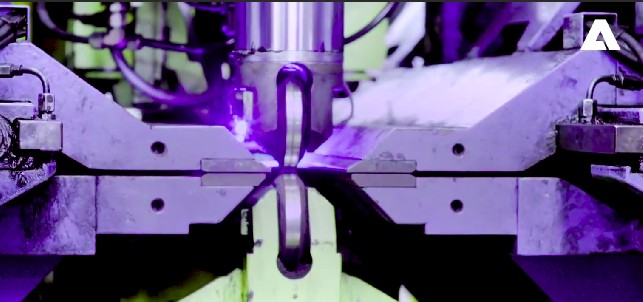
\includegraphics[width=0.90\textwidth]{./Figures/soldadorCO201.jpg}
	\caption{Soldadura con $CO_{2}$ El brillo del láser se encuentra tapado por las ruedas que aplanan el borde de las chapas\protect\footnotemark.}
	\label{fig:soldadora} 
\end{figure}
\footnotetext{\url{https://youtu.be/u6hIaRdXleE?list=PLDD7zo2J8P3fcZPL6RioW2hyscS1Okfh2&t=86}}

En la figura \ref{fig:rayosX} podemos ver la imagen de rayos X de la soldadura por láser de $CO_{2}$ tal como la ve el operador de la cabina de control del tren de laminación.

\begin{figure}[h]
	\centering
	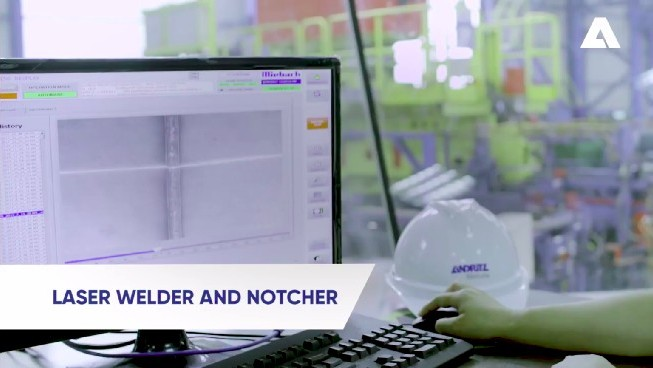
\includegraphics[width=0.90\textwidth]{./Figures/soldaduraCO201.jpg}
	\caption{Rayos X de la soldadura\protect\footnotemark.}
	\label{fig:rayosX} 
\end{figure}
\footnotetext{\url{https://youtu.be/u6hIaRdXleE?list=PLDD7zo2J8P3fcZPL6RioW2hyscS1Okfh2&t=78}}


